% Отчёт о практической работе № 1 «Решение задачи двух тел», вариант 4.
% Оформление — по ГОСТ 7.32-2017 «Отчет о научно-исследовательской работе.
% Структура и правила оформления», список источников — по ГОСТ 7.0.100-2018.
% Сборка: latexmk -xelatex report.tex   (рисунки: python report/make_figures.py)

\documentclass[a4paper,14pt]{extarticle}

% ===================== Данные для титульного листа ==========================
\newcommand{\Ministry}{Министерство науки и высшего образования Российской Федерации}
\newcommand{\Organization}{Федеральное государственное бюджетное образовательное
  учреждение высшего образования\\
  «Национальный исследовательский университет «МЭИ»}
\newcommand{\Institute}{Институт тепловой и атомной энергетики}
\newcommand{\Department}{Кафедра общей физики и ядерного синтеза}
\newcommand{\Discipline}{Имитационное моделирование плазменных процессов}
\newcommand{\StudentName}{Голов~Я.\,А.}
\newcommand{\TeacherName}{Лубенченко~А.\,В.}
\newcommand{\City}{Москва}
\newcommand{\Year}{2026}
% ============================================================================

\usepackage{amsmath,amssymb}
\usepackage{fontspec}
\IfFontExistsTF{Times New Roman}
  {\setmainfont{Times New Roman}}
  {\setmainfont{Liberation Serif}} % метрический аналог Times New Roman
\setmonofont{DejaVu Sans Mono}[Scale=0.85]
\usepackage[russian]{babel}
\usepackage{icomma}

% Поля по ГОСТ 7.32-2017, п. 6.1.1: левое 30, правое 15, верхнее и нижнее 20 мм
\usepackage[left=30mm,right=15mm,top=20mm,bottom=20mm,footskip=10mm]{geometry}
\usepackage{setspace}
\onehalfspacing
\usepackage{indentfirst}
\setlength{\parindent}{1.25cm}
\setlength{\parskip}{0pt}
\usepackage{microtype}
\setlength{\emergencystretch}{3em}

\usepackage{graphicx}
\graphicspath{{figures/}}
\usepackage{float}
\usepackage{array}
\usepackage{tikz}
\usetikzlibrary{arrows.meta,positioning}

% Подписи: «Рисунок 1 – Название» по центру под рисунком,
% «Таблица 1 – Название» слева над таблицей (ГОСТ 7.32-2017, пп. 6.5, 6.6)
\usepackage{caption}
\captionsetup{labelsep=endash, font={stretch=1.5}}
\captionsetup[figure]{name=Рисунок, justification=centering, skip=6pt}
\captionsetup[table]{name=Таблица, justification=raggedright,
  singlelinecheck=false, position=top, skip=6pt}
\addto\captionsrussian{%
  \renewcommand{\figurename}{Рисунок}%
  \renewcommand{\tablename}{Таблица}%
  \renewcommand{\contentsname}{СОДЕРЖАНИЕ}%
}

% Заголовки разделов: с абзацного отступа, полужирные, без точки в конце;
% каждый раздел — с новой страницы (ГОСТ 7.32-2017, п. 6.2)
\usepackage{titlesec}
\titleformat{\section}{\normalfont\bfseries}{\thesection}{0.5em}{}
\titleformat{\subsection}{\normalfont\bfseries}{\thesubsection}{0.5em}{}
\titlespacing*{\section}{\parindent}{0pt}{18pt}
\titlespacing*{\subsection}{\parindent}{18pt}{12pt}
\newcommand{\sectionbreak}{\clearpage}

% Структурные элементы («ВВЕДЕНИЕ», «ЗАКЛЮЧЕНИЕ» и т. д.): по центру, прописными
\newcommand{\structuralelement}[1]{%
  \clearpage\phantomsection
  \addcontentsline{toc}{section}{#1}%
  {\centering\bfseries #1\par}\vspace{18pt}}

% Приложения (ГОСТ 7.32-2017, п. 6.14)
\usepackage{totcount}
\newtotcounter{appendices}
\newcounter{appsub}
\newcommand{\appendixsection}[2]{%
  \clearpage\phantomsection\stepcounter{appendices}\setcounter{appsub}{0}%
  \def\currentappendix{#1}%
  \addcontentsline{toc}{section}{ПРИЛОЖЕНИЕ #1 #2}%
  {\centering\bfseries ПРИЛОЖЕНИЕ #1\par}%
  {\centering (обязательное)\par}%
  {\centering\bfseries #2\par}\vspace{18pt}}
\newcommand{\appendixsubsection}[1]{%
  \stepcounter{appsub}\par\vspace{12pt}%
  {\noindent\hspace*{\parindent}\bfseries\currentappendix.\theappsub\ #1\par}%
  \vspace{6pt}}

\usepackage{tocloft}
\renewcommand{\cfttoctitlefont}{\hfill\bfseries}
\renewcommand{\cftaftertoctitle}{\hfill}
\setlength{\cftbeforetoctitleskip}{0pt}
\setlength{\cftaftertoctitleskip}{18pt}
\renewcommand{\cftsecfont}{\normalfont}
\renewcommand{\cftsecpagefont}{\normalfont}
\renewcommand{\cftsecleader}{\cftdotfill{\cftdotsep}}
\setlength{\cftbeforesecskip}{0pt}

% Перечисления: с абзацного отступа, элементы — через тире (ГОСТ 7.32-2017, п. 6.3.4)
\usepackage{enumitem}
\setlist{nosep}
\setlist[itemize]{label=\textendash, wide=\parindent}
\setlist[enumerate]{label=\arabic*), wide=\parindent}

% Тексты программ: fvextra выводит Unicode без искажений и переносит длинные строки
\usepackage{fvextra}
\fvset{
  fontsize=\footnotesize,
  baselinestretch=1,
  numbers=left,
  numbersep=6pt,
  frame=single,
  breaklines=true,
  breakanywhere=false,
  tabsize=4,
  xleftmargin=18pt,
}
\renewcommand{\theFancyVerbLine}{\tiny\arabic{FancyVerbLine}}

\regtotcounter{figure}
\regtotcounter{table}
\newtotcounter{sources}
\usepackage{lastpage}

\usepackage[hidelinks]{hyperref}

\usepackage{etoolbox}
% Ссылка на один или несколько источников: [1] или [1, 2]
\newcommand{\citeitem}[1]{\citesep\ref{#1}\def\citesep{,~}}
\newcommand{\cit}[1]{[\def\citesep{}\forcsvlist{\citeitem}{#1}]}
% Строки таблиц, сформированные make_figures.py (примитив \input не создает
% лишнюю строку в tabular)
\makeatletter
\newcommand{\inputrows}[1]{\@@input #1 }
\makeatother
\newcommand{\eV}{\text{эВ}}
\newcommand{\nm}{\text{нм}}

\begin{document}

% =============================== ТИТУЛЬНЫЙ ЛИСТ ==============================
\begin{titlepage}
  \setstretch{1}
  \begin{center}
    \Ministry\\[6pt]
    \Organization\\[12pt]
    \Institute\\[6pt]
    \Department
  \end{center}

  \vfill

  \begin{center}
    {\bfseries ОТЧЕТ\\
    О ПРАКТИЧЕСКОЙ РАБОТЕ № 1}\\[12pt]
    по дисциплине «\Discipline»\\[24pt]
    {\bfseries РЕШЕНИЕ ЗАДАЧИ ДВУХ ТЕЛ}\\[12pt]
    Вариант 4
  \end{center}

  \vfill

  \noindent
  \begin{tabular}{@{}p{7.5cm}>{\raggedleft\arraybackslash}p{7.5cm}@{}}
    Студент       & \StudentName \\[12pt]
    Преподаватель & \TeacherName \\
  \end{tabular}

  \vfill

  \begin{center}
    \City\ \Year
  \end{center}
\end{titlepage}
\setcounter{page}{2}

% ================================== РЕФЕРАТ ==================================
\clearpage
{\centering\bfseries РЕФЕРАТ\par}\vspace{18pt}

Отчет \pageref{LastPage}~с., \total{figure}~рис., \total{table}~табл.,
\total{sources}~источн., \total{appendices}~прил.

ЗАДАЧА ДВУХ ТЕЛ, УПРУГОЕ РАССЕЯНИЕ, ЭКРАНИРОВАННЫЙ КУЛОНОВСКИЙ ПОТЕНЦИАЛ,
ПОТЕНЦИАЛ KR-C, РАДИУС ЭКРАНИРОВАНИЯ ФИРСОВА, ПРИЦЕЛЬНЫЙ ПАРАМЕТР,
КИНЕМАТИЧЕСКИЙ ФАКТОР, КВАДРАТУРА ГАУССА~--~МЕЛЕРА, ДИФФЕРЕНЦИАЛЬНОЕ СЕЧЕНИЕ
РАССЕЯНИЯ

Объектом исследования является упругое парное столкновение протона
с покоящимся атомом меди при энергии налетающей частицы 0,1~эВ.

Цель работы~--- определение зависимости угла рассеяния частицы от прицельного
параметра при столкновении двух частиц и зависимости дифференциального сечения
упругого рассеяния от углов рассеяния.

Методы исследования: классическая теория рассеяния двух тел
с экранированным кулоновским потенциалом Kr-C, численное решение нелинейного
уравнения методом деления отрезка пополам, численное интегрирование методом
Гаусса~--~Мелера, численное дифференцирование. Программа написана на языке
Python с применением объектно"=ориентированного подхода.

В результате работы рассчитаны зависимости потенциальной энергии
взаимодействия от расстояния, кинематического фактора и энергии рассеянной
частицы от угла рассеяния, расстояния наименьшего сближения, угла рассеяния
в системе центра масс и углов рассеяния в лабораторной системе отсчета от
прицельного параметра, а также дифференциальные сечения упругого рассеяния.
Правильность программы подтверждена сравнением с точным решением задачи
рассеяния в кулоновском поле.

Результаты могут быть использованы при моделировании взаимодействия
ионов с веществом методами молекулярной динамики и Монте-Карло.

% ================================ СОДЕРЖАНИЕ =================================
\clearpage
\tableofcontents

% ================================= ВВЕДЕНИЕ ==================================
\structuralelement{ВВЕДЕНИЕ}

Расчет парных столкновений лежит в основе имитационного моделирования
взаимодействия ускоренных частиц с веществом: и в методе молекулярной
динамики, и в методе Монте-Карло результат отдельного столкновения
определяется углом рассеяния и потерей энергии, которые зависят от потенциала
взаимодействия и прицельного параметра~\cit{ref:manual}.

Цель работы~--- определение зависимости угла рассеяния частицы от прицельного
параметра при столкновении двух частиц и зависимости дифференциального сечения
упругого рассеяния от углов рассеяния.

Задание: рассчитать зависимости угла рассеяния в системе центра масс от
прицельного параметра, зависимости углов рассеяния в лабораторной системе
отсчета от прицельного параметра, зависимости дифференциального сечения
упругого рассеяния от углов рассеяния в лабораторной системе отсчета.
При расчете взаимодействия ионов использовать экранированные потенциалы
рассеяния.

Исходные данные варианта~4 (сочетание вариантов А\,=\,3 и Б\,=\,1)
приведены в таблице~\ref{tab:variant}.

\begin{table}[H]
  \caption{Исходные данные варианта 4}
  \label{tab:variant}
  \setstretch{1}
  \begin{tabular}{|p{8cm}|p{7.2cm}|}
    \hline
    Параметр & Значение \\ \hline
    Потенциал взаимодействия & Kr-C \\ \hline
    Радиус экранирования & Фирсова \\ \hline
    Энергия налетающей частицы $E_0$, эВ & 0,1 \\ \hline
    Налетающая частица & протон p ($Z_1 = 1$, $m_1 = 1{,}00728$~а.\,е.\,м.) \\ \hline
    Покоящаяся частица & атом меди Cu ($Z_2 = 29$, $m_2 = 63{,}546$~а.\,е.\,м.) \\ \hline
  \end{tabular}
\end{table}

Для достижения цели необходимо решить следующие задачи:
\begin{itemize}
  \item построить зависимость потенциальной энергии взаимодействия $U(r)$
        от расстояния между частицами;
  \item рассчитать зависимости кинематического фактора $k$ и энергии
        налетающей частицы после рассеяния $E_1$ от угла рассеяния $\theta_1$;
  \item рассчитать зависимость расстояния наименьшего сближения $R$ от
        прицельного параметра $\rho$ и построить сетку прицельных параметров;
  \item рассчитать зависимость угла рассеяния в системе центра масс $\chi$
        и углов рассеяния в лабораторной системе $\theta_1$, $\theta_2$
        от прицельного параметра;
  \item рассчитать дифференциальные сечения упругого рассеяния
        $\omega(\theta_1)$ и $\omega(\theta_2)$;
  \item разработать программу на языке Python с применением
        объектно"=ориентированного подхода и проверить ее на тестовой задаче.
\end{itemize}

% ============================ 1 ФИЗИЧЕСКАЯ МОДЕЛЬ ============================
\section{Физическая модель}

Рассматривается упругое столкновение двух частиц: налетающей частицы
массой $m_1$ с кинетической энергией $E_0$ и покоящейся частицы-мишени массой
$m_2$. Принимаются следующие допущения~\cit{ref:manual,ref:landau,ref:eckstein}:
\begin{itemize}
  \item внешние силы на систему не действуют, поэтому выполняются законы
        сохранения энергии, импульса и момента импульса;
  \item потенциал взаимодействия зависит только от расстояния между
        частицами, поэтому движение происходит в одной плоскости;
  \item потери энергии на возбуждение и ионизацию электронных оболочек
        (неупругие потери) не учитываются;
  \item движение частиц описывается классической механикой.
\end{itemize}

Применимость классического описания оценивается по длине волны де Бройля
налетающей частицы~\cit{ref:manual}. Для протона с энергией 0,1~эВ
$\lambda_\text{Б} = 2{,}87\cdot 10^{-2} / \sqrt{M E_0} \approx 0{,}09$~нм,
что в три раза меньше расстояния наименьшего сближения при лобовом
столкновении ($\approx 0{,}28$~нм, см. раздел~\ref{sec:results}).
Следовательно, вариант задания находится вблизи нижней границы применимости
классического подхода, но не выходит за нее.

Расстояние наименьшего сближения частиц при рассматриваемых энергиях
велико по сравнению с размерами ядер, поэтому важную роль играет
экранирование заряда ядер электронными оболочками. Взаимодействие
описывается экранированным кулоновским потенциалом~--- кулоновским
потенциалом ядер, умноженным на функцию экранирования, которая учитывает
действие электронных оболочек.

Задача двух тел сводится к задаче о движении одной частицы с приведенной
массой $\mu = m_1 m_2 / (m_1 + m_2)$ в центральном поле $U(r)$.
Угол рассеяния в системе центра масс (ц-системе) определяется потенциалом,
относительной энергией и прицельным параметром~$\rho$; углы рассеяния
в лабораторной системе (л-системе), связанной с покоящейся до удара мишенью,
находятся из кинематических соотношений. Для пучка частиц с равномерным
распределением по прицельным параметрам вероятность рассеяния в заданный
телесный угол характеризуется дифференциальным сечением рассеяния.

% =========================== 2 МАТЕМАТИЧЕСКАЯ МОДЕЛЬ ==========================
\section{Математическая модель}

\subsection{Потенциал взаимодействия}

Потенциальная энергия взаимодействия частиц описывается экранированным
кулоновским потенциалом~\cit{ref:manual}
\begin{equation}
  U(r) = \frac{Z_1 Z_2 e^2}{r}\, F\!\left(\frac{r}{a}\right),
  \label{eq:potential}
\end{equation}
где $Z_1$, $Z_2$~--- порядковые номера налетающей частицы и мишени;

$e^2 = 1{,}44$~эВ$\cdot$нм~--- квадрат элементарного заряда;

$r$~--- расстояние между частицами, нм;

$F$~--- функция экранирования;

$a$~--- длина (радиус) экранирования, нм.

Функция экранирования представляется суммой экспонент
\begin{equation}
  F(x) = \sum_{i=1}^{n} c_i \exp(-d_i x), \qquad \sum_{i=1}^{n} c_i = 1,
  \label{eq:screening}
\end{equation}
где $c_i$, $d_i$~--- константы потенциала.

Для потенциала Kr-C~\cit{ref:krc} $n = 3$, константы приведены
в таблице~\ref{tab:krc}.

\begin{table}[H]
  \caption{Константы функции экранирования потенциала Kr-C}
  \label{tab:krc}
  \setstretch{1}
  \centering
  \begin{tabular}{|c|c|c|}
    \hline
    $i$ & $c_i$ & $d_i$ \\ \hline
    1 & 0,190945 & 0,278544 \\ \hline
    2 & 0,473674 & 0,637174 \\ \hline
    3 & 0,335381 & 1,919249 \\ \hline
  \end{tabular}
\end{table}

Радиус экранирования Фирсова~\cit{ref:manual}
\begin{equation}
  a_\text{Ф} = \left(\frac{9\pi^2}{128}\right)^{1/3} a_\text{Б}
  \left(Z_1^{1/2} + Z_2^{1/2}\right)^{-2/3}
  \approx 0{,}8853\, a_\text{Б}\left(Z_1^{1/2} + Z_2^{1/2}\right)^{-2/3},
  \label{eq:firsov}
\end{equation}
где $a_\text{Б} = 0{,}0529$~нм~--- первый боровский радиус.

Для пары p~--~Cu $a_\text{Ф} = 0{,}013608$~нм.

\subsection{Кинематика упругого столкновения}

Из законов сохранения энергии и импульса следует выражение для
кинематического фактора~--- отношения энергии налетающей частицы после
рассеяния $E_1$ к начальной энергии~\cit{ref:manual,ref:landau}:
\begin{equation}
  k(\theta_1) = \frac{E_1}{E_0} = \left(\frac{m_1}{m_1 + m_2}\right)^2
  \left(\cos\theta_1 + \sqrt{\left(\frac{m_2}{m_1}\right)^2 - \sin^2\theta_1}\right)^2,
  \label{eq:kinematic}
\end{equation}
где $\theta_1$~--- угол рассеяния налетающей частицы в л-системе.

Так как $m_1 < m_2$, угол $\theta_1$ может принимать любые значения от 0 до
$\pi$, а энергия после рассеяния $E_1 = k E_0$ изменяется от $E_0$ до
$E_0 \left((m_2 - m_1)/(m_1 + m_2)\right)^2$.

Энергия относительного движения (энергия в ц-системе)
\begin{equation}
  E_r = E_0\, \frac{m_2}{m_1 + m_2}.
  \label{eq:er}
\end{equation}

Для варианта~4 $E_r = 0{,}098440$~эВ.

\subsection{Угол рассеяния и сечение}

Угол рассеяния в ц-системе~\cit{ref:manual,ref:landau}
\begin{equation}
  \chi(\rho) = \pi - 2\rho \int\limits_R^{\infty} \frac{dr}{r^2\sqrt{g(r)}},
  \qquad
  g(r) = 1 - \frac{U(r)}{E_r} - \frac{\rho^2}{r^2},
  \label{eq:chi}
\end{equation}
где $\rho$~--- прицельный параметр, нм;

$R$~--- расстояние наименьшего сближения, нм, определяемое как наибольший
корень уравнения
\begin{equation}
  g(R) = 1 - \frac{U(R)}{E_r} - \frac{\rho^2}{R^2} = 0.
  \label{eq:closest}
\end{equation}

Углы рассеяния налетающей частицы $\theta_1$ и частицы отдачи $\theta_2$
в л-системе связаны с углом $\chi$ соотношениями
\begin{equation}
  \operatorname{tg}\theta_1 = \frac{m_2 \sin\chi}{m_1 + m_2 \cos\chi},
  \qquad
  \theta_2 = \frac{\pi - \chi}{2}.
  \label{eq:lab}
\end{equation}

Дифференциальное сечение упругого рассеяния
\begin{equation}
  \omega(\theta) = \frac{\rho(\theta)}{\sin\theta}
  \left|\frac{d\rho(\theta)}{d\theta}\right|,
  \label{eq:sigma}
\end{equation}
где $\rho(\theta)$~--- функция, обратная зависимости угла рассеяния
от прицельного параметра;

$\theta$~--- угол рассеяния $\theta_1$ или $\theta_2$.

% ===================== 3 ДИСКРЕТНАЯ МОДЕЛЬ И АЛГОРИТМ =========================
\section{Дискретная модель и алгоритм решения}

\subsection{Расстояние наименьшего сближения}

Для отталкивающего потенциала~\eqref{eq:potential} оба слагаемых
$-U(r)/E_r$ и $-\rho^2/r^2$ монотонно возрастают с ростом $r$, поэтому
функция $g(r)$ монотонно возрастает от $-\infty$ при $r \to 0$ до 1 при
$r \to \infty$, и уравнение~\eqref{eq:closest} имеет единственный корень.
Корень находится методом деления отрезка пополам:
\begin{enumerate}
  \item начальная правая граница $r_+ = \max(\rho, 10^{-3}~\text{нм})$
        удваивается, пока $g(r_+) < 0$;
  \item начальная левая граница $r_- = r_+$ уменьшается вдвое, пока
        $g(r_-) \geqslant 0$;
  \item отрезок $[r_-, r_+]$ делится пополам до достижения относительной
        точности $10^{-14}$; в качестве $R$ принимается правая граница,
        на которой $g(R) \geqslant 0$, что гарантирует неотрицательность
        подкоренного выражения в~\eqref{eq:chi}.
\end{enumerate}

\subsection{Сетка прицельных параметров}

При больших прицельных параметрах потенциал не влияет на движение частиц
и $R \to \rho$. Максимальный прицельный параметр $\rho_{\max}$~--- наименьшее
значение, при котором
\begin{equation}
  \left|1 - \frac{R(\rho_{\max})}{\rho_{\max}}\right| < 10^{-3}.
  \label{eq:rhomax}
\end{equation}

Величина $|1 - R/\rho|$ монотонно убывает с ростом $\rho$, поэтому
$\rho_{\max}$ находится так же, как корень~\eqref{eq:closest}: начиная
с $\rho = R(0)$, прицельный параметр удваивается до выполнения
условия~\eqref{eq:rhomax}, после чего граница уточняется делением отрезка
пополам. Сетка прицельных параметров
\begin{equation}
  \rho_j = j\,\Delta\rho, \qquad \Delta\rho = \frac{\rho_{\max}}{200},
  \qquad j = 1, 2, \ldots, 200.
  \label{eq:grid}
\end{equation}

\subsection{Численное интегрирование}

Подынтегральная функция в~\eqref{eq:chi} имеет интегрируемую особенность
в точке $r = R$, где $g(R) = 0$. Замена переменной $r = R/\xi^2$
переводит интеграл на отрезок $\xi \in [0, 1]$, а последующая замена
$\xi = \cos\psi$ устраняет особенность. Применение к полученному интегралу
квадратурной формулы средних прямоугольников по $\psi$ дает формулу
Гаусса~--~Мелера~\cit{ref:manual}
\begin{equation}
  \chi = \pi - 2\,\frac{\rho}{R}\,\frac{\pi}{N}
  \sum_{n=1}^{N} \frac{\xi_n \xi_{N-n+1}}{\sqrt{g\left(R/\xi_n^2\right)}},
  \qquad
  \xi_n = \cos\frac{(2n - 1)\pi}{4N},
  \label{eq:gauss}
\end{equation}
где $N$~--- число узлов квадратуры; в расчетах $N = 100$.

\subsection{Численное дифференцирование}

Зависимости $\rho(\theta_1)$ и $\rho(\theta_2)$ получаются обращением
табличных зависимостей $\theta_1(\rho_j)$, $\theta_2(\rho_j)$: значения
упорядочиваются по возрастанию угла. Сетка по углу неравномерная,
поэтому производная в~\eqref{eq:sigma} вычисляется по центральной
разностной формуле второго порядка для неравномерной сетки
\begin{equation}
  \left.\frac{d\rho}{d\theta}\right|_{j} \approx
  \frac{h_{j-1}^2 \rho_{j+1} - h_j^2 \rho_{j-1} + \left(h_j^2 - h_{j-1}^2\right)\rho_j}
       {h_{j-1} h_j \left(h_{j-1} + h_j\right)},
  \label{eq:derivative}
\end{equation}
где $h_{j-1} = \theta_j - \theta_{j-1}$, $h_j = \theta_{j+1} - \theta_j$~---
шаги сетки по углу.

На концах сетки используются односторонние разности первого порядка.

\subsection{Алгоритм решения}

Расчет выполняется в следующем порядке:
\begin{enumerate}
  \item по таблицам вариантов формируются параметры частиц, функция
        и радиус экранирования, вычисляются $a_\text{Ф}$ и $E_r$
        по формулам~\eqref{eq:firsov} и~\eqref{eq:er};
  \item находятся $\rho_{\max}$ и сетка~\eqref{eq:grid}, для каждого узла
        сетки решается уравнение~\eqref{eq:closest};
  \item на логарифмической сетке расстояний от $R_{\min}/10$ до
        $2\rho_{\max}$ вычисляется потенциальная энергия~\eqref{eq:potential};
  \item на сетке углов $\theta_1 \in [0, \pi]$ из 361 точки вычисляются
        $k(\theta_1)$ и $E_1(\theta_1)$ по формуле~\eqref{eq:kinematic};
  \item для каждого узла сетки прицельных параметров вычисляется угол
        $\chi$ по формуле~\eqref{eq:gauss} и углы $\theta_1$, $\theta_2$
        по формулам~\eqref{eq:lab};
  \item вычисляются сечения $\omega(\theta_1)$ и $\omega(\theta_2)$
        по формулам~\eqref{eq:sigma} и~\eqref{eq:derivative};
  \item результаты выводятся в виде таблицы и графиков.
\end{enumerate}

% ========================= 4 ПРОГРАММНАЯ РЕАЛИЗАЦИЯ ===========================
\section{Программная реализация}

Программа написана на языке Python~3~\cit{ref:python} с использованием
библиотек NumPy~\cit{ref:numpy} (векторные вычисления) и
Matplotlib~\cit{ref:matplotlib} (построение графиков). Программа построена
на принципах объектно"=ориентированного программирования: каждая физическая
сущность и каждый численный метод представлены отдельным классом, общие
свойства вынесены в абстрактные базовые классы. Это позволяет менять
потенциал, радиус экранирования или пару частиц без изменения алгоритма
расчета. Назначение классов приведено в таблице~\ref{tab:classes},
связи между ними показаны на рисунке~\ref{fig:classes}. Текст программы
приведен в приложении~А.

\begin{table}[H]
  \caption{Классы программы}
  \label{tab:classes}
  \setstretch{1}
  \small
  \begin{tabular}{|p{5.9cm}|p{9.3cm}|}
    \hline
    Класс & Назначение \\ \hline
    \texttt{Particle}, \texttt{ParticleCatalog} &
      Частица (заряд ядра, масса) и справочник частиц \\ \hline
    \texttt{ScreeningFunction} &
      Функция экранирования~\eqref{eq:screening}; экземпляры
      \texttt{BOHR}, \texttt{MOLIERE}, \texttt{KR\_C}, \texttt{ZBL} \\ \hline
    \texttt{ScreeningLength} (абстрактный) &
      Радиус экранирования $a(Z_1, Z_2)$ \\ \hline
    \texttt{ThomasFermiScreeningLength} &
      Радиус экранирования модели Томаса~--~Ферми
      $a = 0{,}8853\,a_\text{Б}\,Z_{12}^{-1/3}$,
      $Z_{12} = (Z_1^x + Z_2^x)^y$ \\ \hline
    \texttt{FirsovScreeningLength}, \texttt{LindhardScharff}\allowbreak\texttt{ScreeningLength},
    \texttt{ZBLScreeningLength} &
      Радиусы экранирования Фирсова, Линдхарда~--~Шарфа и ZBL \\ \hline
    \texttt{InteractionPotential} (абстрактный) &
      Потенциальная энергия взаимодействия $U(r)$ \\ \hline
    \texttt{CoulombPotential}, \texttt{ScreenedCoulombPotential} &
      Кулоновский и экранированный кулоновский~\eqref{eq:potential}
      потенциалы \\ \hline
    \texttt{BinaryCollision} &
      Кинематика столкновения: $E_r$, $k(\theta_1)$, $E_1(\theta_1)$,
      пересчет $\chi$ в $\theta_1$, $\theta_2$ \\ \hline
    \texttt{RadialFunction} & Функция $g(r)$ из~\eqref{eq:chi} \\ \hline
    \texttt{ClosestApproachSolver} &
      Решение уравнения~\eqref{eq:closest} \\ \hline
    \texttt{ImpactParameterGrid} &
      Поиск $\rho_{\max}$ и построение сетки~\eqref{eq:grid} \\ \hline
    \texttt{GaussMehlerScatteringAngle} &
      Угол рассеяния по формуле~\eqref{eq:gauss} \\ \hline
    \texttt{DifferentialCrossSection} &
      Сечение рассеяния~\eqref{eq:sigma} \\ \hline
    \texttt{Variant} &
      Вариант задания и создание объектов задачи по таблицам вариантов \\ \hline
    \texttt{TwoBodyScatteringExperiment}, \texttt{ScatteringResults} &
      Выполнение расчета и хранение результатов \\ \hline
    \texttt{ResultsPlotter} & Построение графиков \\ \hline
    \texttt{Application} & Консольный запуск программы \\ \hline
  \end{tabular}
\end{table}

\begin{figure}[H]
  \centering
  \setstretch{1}
  \begin{tikzpicture}[
      font=\footnotesize,
      cls/.style={draw, rectangle, minimum height=6mm, inner sep=2.5pt, align=center},
      abs/.style={cls, font=\footnotesize\itshape},
      inherit/.style={-{Triangle[open,length=2.4mm,width=2.4mm]}},
      uses/.style={-{Stealth[length=1.8mm]}, dashed},
    ]
    % Экранирование и потенциалы
    \node[abs] (SL)  at (-2.5, 0)    {ScreeningLength};
    \node[cls] (TF)  at (-5.0, -1.4) {ThomasFermiScreeningLength};
    \node[cls] (ZBL) at (-0.8, -1.4) {ZBLScreeningLength};
    \node[cls] (FIR) at (-6.4, -2.8) {FirsovScreeningLength};
    \node[cls] (LS)  at (-1.9, -2.8) {LindhardScharffScreeningLength};
    \node[cls] (SF)  at (3.0, -1.4)  {ScreeningFunction};
    \node[abs] (IP)  at (6.2, 0)     {InteractionPotential};
    \node[cls] (CP)  at (6.2, -1.4)  {CoulombPotential};
    \node[cls] (SCP) at (6.2, -2.8)  {ScreenedCoulombPotential};
    \draw[inherit] (TF) -- (SL);
    \draw[inherit] (ZBL) -- (SL);
    \draw[inherit] (FIR) -- (TF);
    \draw[inherit] (LS) -- (TF);
    \draw[inherit] (CP) -- (IP);
    \draw[inherit] (SCP) -- (CP);
    \draw[uses] (SCP.north west) -- (SCP.north west |- SF.south);
    \draw[uses] (SCP.west) -- (1.25, -2.8) -- (1.25, 0) -- (SL.east);

    % Частицы, вариант, кинематика
    \node[cls] (P)   at (-7.3, -4.3) {Particle};
    \node[cls] (PC)  at (-4.6, -4.3) {ParticleCatalog};
    \node[cls] (BC)  at (-0.9, -4.3) {BinaryCollision};
    \node[cls] (V)   at (2.8, -4.3)  {Variant};
    \draw[uses] (PC) -- (P);
    \draw[uses] (BC) -- (PC);
    \draw[uses] (V) -- (BC);
    \draw[uses] (V.north) -- (SCP.south west);

    % Численные методы
    \node[cls] (RF)  at (-7.0, -5.8) {RadialFunction};
    \node[cls] (CAS) at (-3.6, -5.8) {ClosestApproachSolver};
    \node[cls] (IPG) at (0.0, -5.8)  {ImpactParameterGrid};
    \node[cls] (GM)  at (5.8, -5.8)  {GaussMehlerScatteringAngle};
    \draw[uses] (CAS) -- (RF);
    \draw[uses] (IPG) -- (CAS);

    % Эксперимент и вывод
    \node[cls] (EXP) at (0.0, -7.3)  {TwoBodyScatteringExperiment};
    \node[cls] (DCS) at (-5.6, -7.3) {DifferentialCrossSection};
    \node[cls] (RES) at (6.0, -7.3)  {ScatteringResults};
    \node[cls] (APP) at (-2.5, -8.8) {Application};
    \node[cls] (PL)  at (2.5, -8.8)  {ResultsPlotter};
    \draw[uses] (EXP) -- (DCS);
    \draw[uses] (EXP) -- (RES);
    \draw[uses] (EXP.north west) -- (CAS.south);
    \draw[uses] (EXP.north) -- (IPG.south);
    \draw[uses] (EXP.east) -- (GM.south);
    \draw[uses] ([xshift=-6mm]EXP.north east) -- (V.south);
    \draw[uses] (APP) -- (EXP);
    \draw[uses] (APP) -- (PL);
    \draw[uses] (PL) -- (RES);
  \end{tikzpicture}

  \vspace{6pt}
  \parbox{15cm}{\footnotesize\setstretch{1}
    Курсивом обозначены абстрактные классы; сплошная линия с треугольником~---
    наследование, штриховая линия со стрелкой~--- использование (ассоциация).}
  \caption{Диаграмма классов программы}
  \label{fig:classes}
\end{figure}

Программа запускается командой \texttt{python main.py} (по умолчанию
выполняется расчет варианта~4, номер варианта задается параметром
\texttt{-{}-variant}). Результаты сохраняются в каталог
\texttt{results/variant\_04}: шесть графиков и таблица значений $\rho$, $R$,
$\chi$, $\theta_1$, $\theta_2$ в формате CSV.

% =========================== 5 ТЕСТОВЫЕ РАСЧЕТЫ ==============================
\section{Тестовые расчеты}
\label{sec:tests}

Для проверки программы использовалось рассеяние в кулоновском поле
($F \equiv 1$), для которого известно точное решение~\cit{ref:landau}:
\begin{equation}
  R(\rho) = \frac{b}{2} + \sqrt{\frac{b^2}{4} + \rho^2},
  \qquad
  \chi(\rho) = 2\operatorname{arctg}\frac{b}{2\rho},
  \qquad
  \omega(\chi) = \left(\frac{b}{4}\right)^2 \frac{1}{\sin^4(\chi/2)},
  \label{eq:rutherford}
\end{equation}
где $b = Z_1 Z_2 e^2 / E_r$~--- расстояние наименьшего сближения при
лобовом столкновении, нм.

Тестовый расчет выполнен для $Z_1 = 1$, $Z_2 = 29$, $E_r = 100$~эВ
($b = 0{,}4176$~нм) на 200 значениях прицельного параметра
от $0{,}01\,b$ до $2\,b$. Получены следующие результаты:
\begin{itemize}
  \item максимальная относительная погрешность расстояния наименьшего
        сближения не превышает $10^{-14}$;
  \item угол рассеяния, рассчитанный по формуле~\eqref{eq:gauss} при
        $N = 100$, совпадает с точным значением с погрешностью не более
        $3{,}2\cdot 10^{-5}$~рад (рисунок~\ref{fig:test}, слева);
  \item относительная погрешность дифференциального сечения во внутренних
        узлах сетки не превышает 0,25~\%, в крайних узлах, где
        используются односторонние разности,~--- 2~\%.
\end{itemize}

\begin{figure}[H]
  \centering
  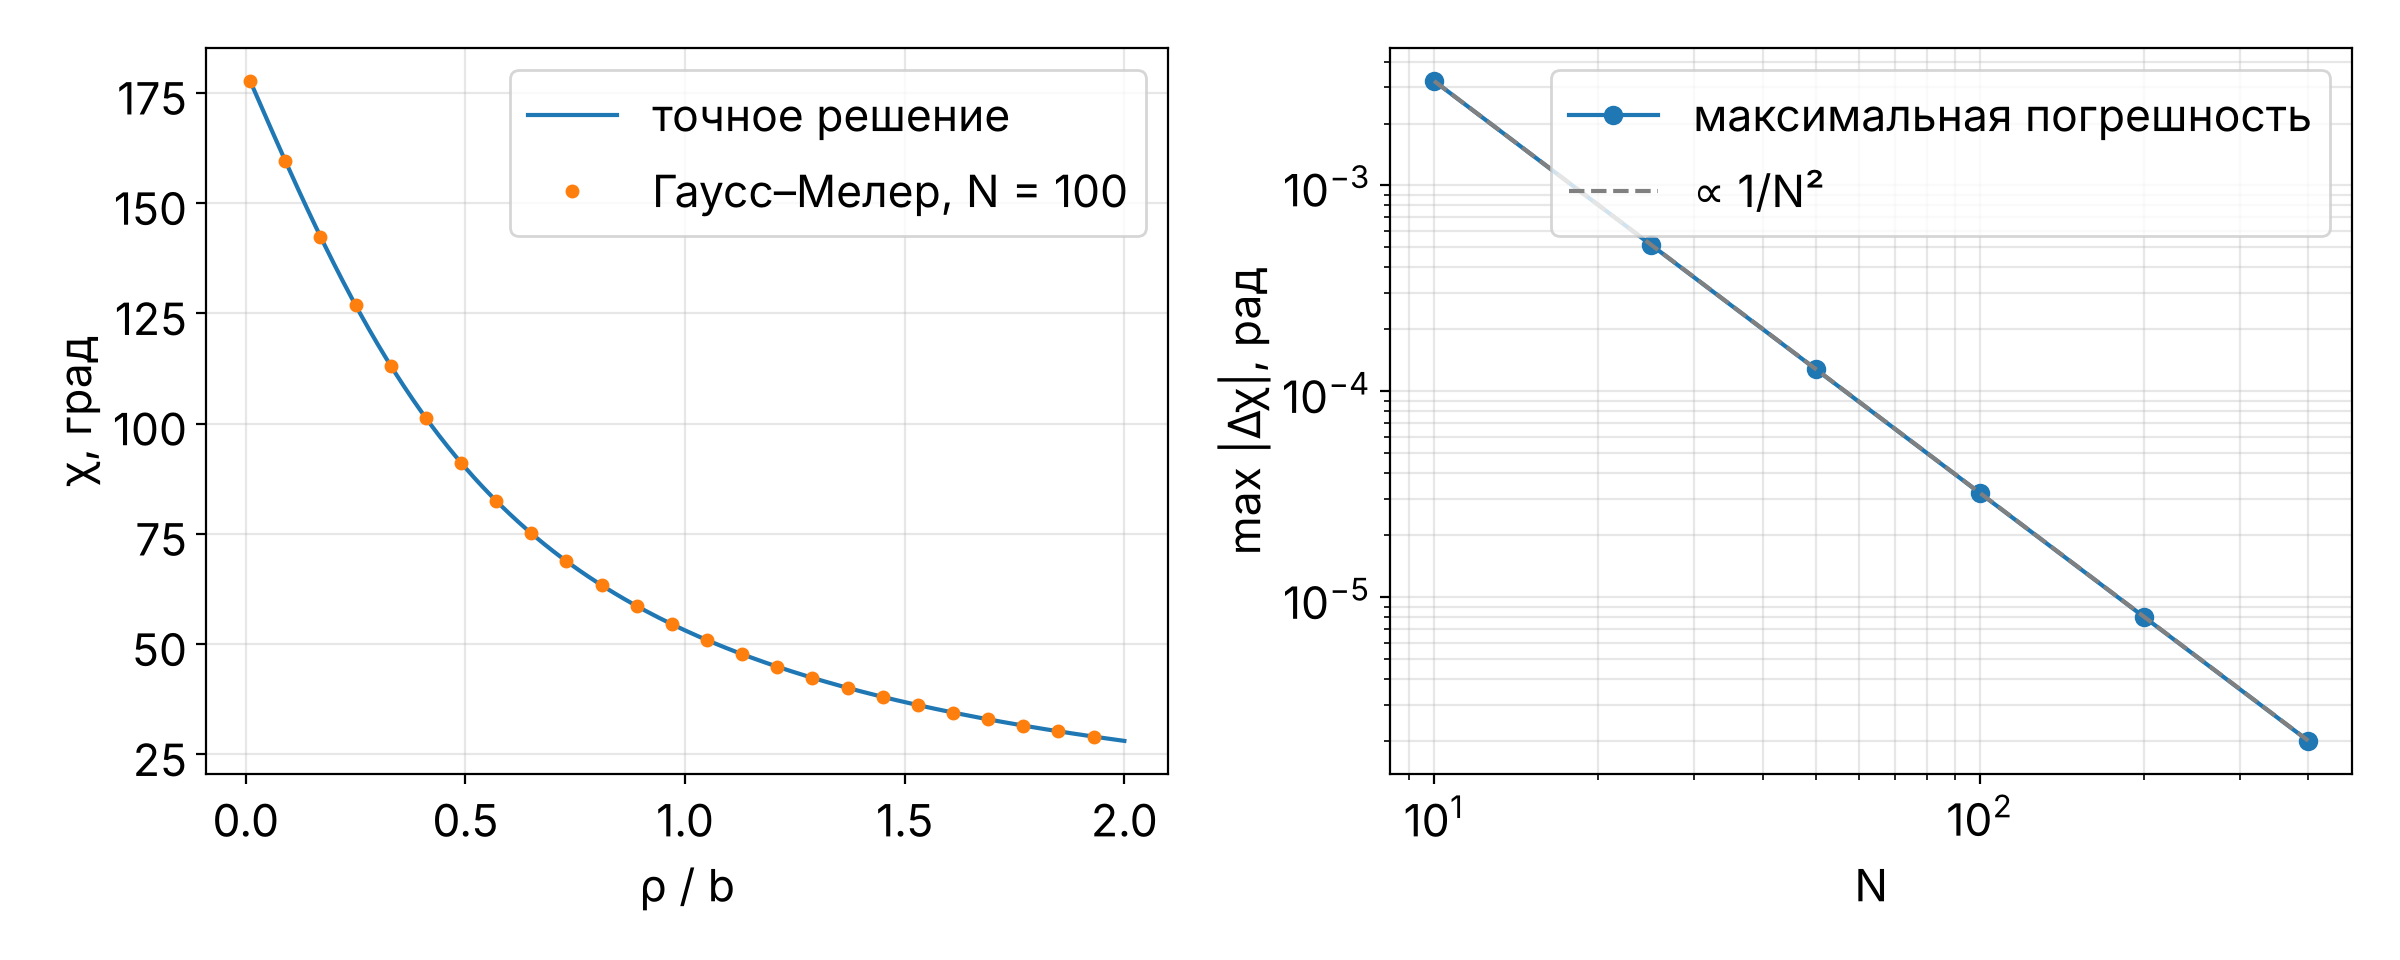
\includegraphics[width=\linewidth]{test_coulomb.png}
  \caption{Угол рассеяния в кулоновском поле (слева) и зависимость
    погрешности формулы Гаусса~--~Мелера от числа узлов (справа)}
  \label{fig:test}
\end{figure}

Зависимость погрешности угла рассеяния от числа узлов $N$ приведена
в таблице~\ref{tab:convergence}. Для варианта~4 погрешность оценивалась
по сравнению с расчетом при $N = 1600$. Погрешность убывает
пропорционально $1/N^2$, что соответствует второму порядку точности
формулы средних прямоугольников. При $N = 100$ погрешность угла рассеяния
не превышает $5\cdot 10^{-5}$~рад ($0{,}003^\circ$), что достаточно для
решаемой задачи.

\begin{table}[H]
  \caption{Максимальная погрешность угла рассеяния $\chi$, рад, в зависимости
    от числа узлов квадратуры}
  \label{tab:convergence}
  \setstretch{1}
  \centering
  \begin{tabular}{|c|c|c|}
    \hline
    $N$ & Кулоновский потенциал & Вариант 4 (Kr-C) \\ \hline
    \inputrows{generated/convergence_rows.tex}
  \end{tabular}
\end{table}

Кроме того, проверены предельные значения кинематического фактора
$k(0) = 1$ и $k(\pi) = \left((m_2 - m_1)/(m_1 + m_2)\right)^2$, выполнение
закона сохранения энергии $E_1 + E_2 = E_0$ при пересчете углов
по формулам~\eqref{eq:lab} и нормировка функций экранирования $F(0) = 1$.
Все тесты (модуль \texttt{tests/test\_two\_body.py}, приложение~А)
выполняются успешно.

% ======================= 6 РЕЗУЛЬТАТЫ МОДЕЛИРОВАНИЯ ==========================
\section{Результаты моделирования}
\label{sec:results}

\subsection{Потенциальная энергия и кинематический фактор}

Зависимость потенциальной энергии взаимодействия протона с атомом меди
от расстояния приведена на рисунке~\ref{fig:potential}. Горизонтальной
линией отмечена энергия относительного движения $E_r = 0{,}0984$~эВ.
Потенциальная энергия становится равной $E_r$ на расстоянии
$R(0) = 0{,}2774$~нм $\approx 20\,a_\text{Ф}$; это расстояние наименьшего
сближения при лобовом столкновении.

\begin{figure}[H]
  \centering
  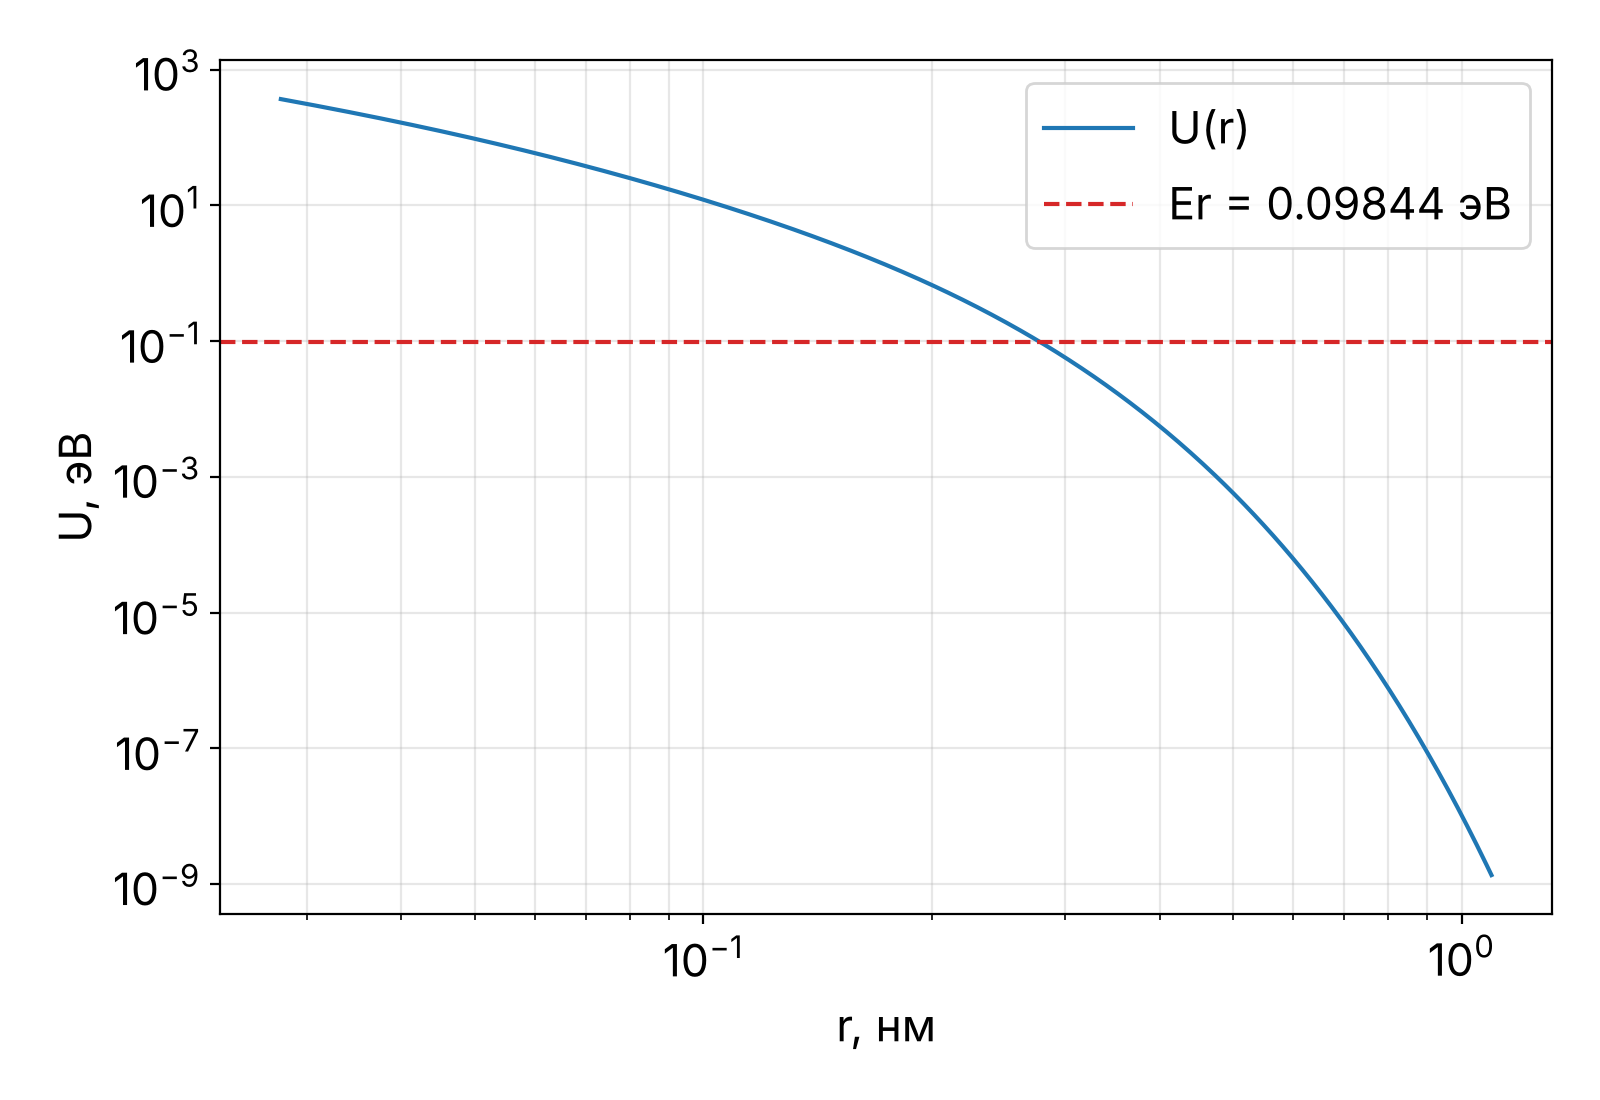
\includegraphics[width=0.85\linewidth]{1a_potential.png}
  \caption{Потенциальная энергия взаимодействия p~--~Cu (потенциал Kr-C,
    радиус экранирования Фирсова)}
  \label{fig:potential}
\end{figure}

Зависимости кинематического фактора и энергии протона после рассеяния
от угла рассеяния приведены на рисунке~\ref{fig:kinematic}.
Кинематический фактор убывает от 1 при $\theta_1 = 0$ до 0,9386 при
$\theta_1 = 180^\circ$; энергия рассеянного протона изменяется от 0,1
до 0,0939~эВ.

\begin{figure}[H]
  \centering
  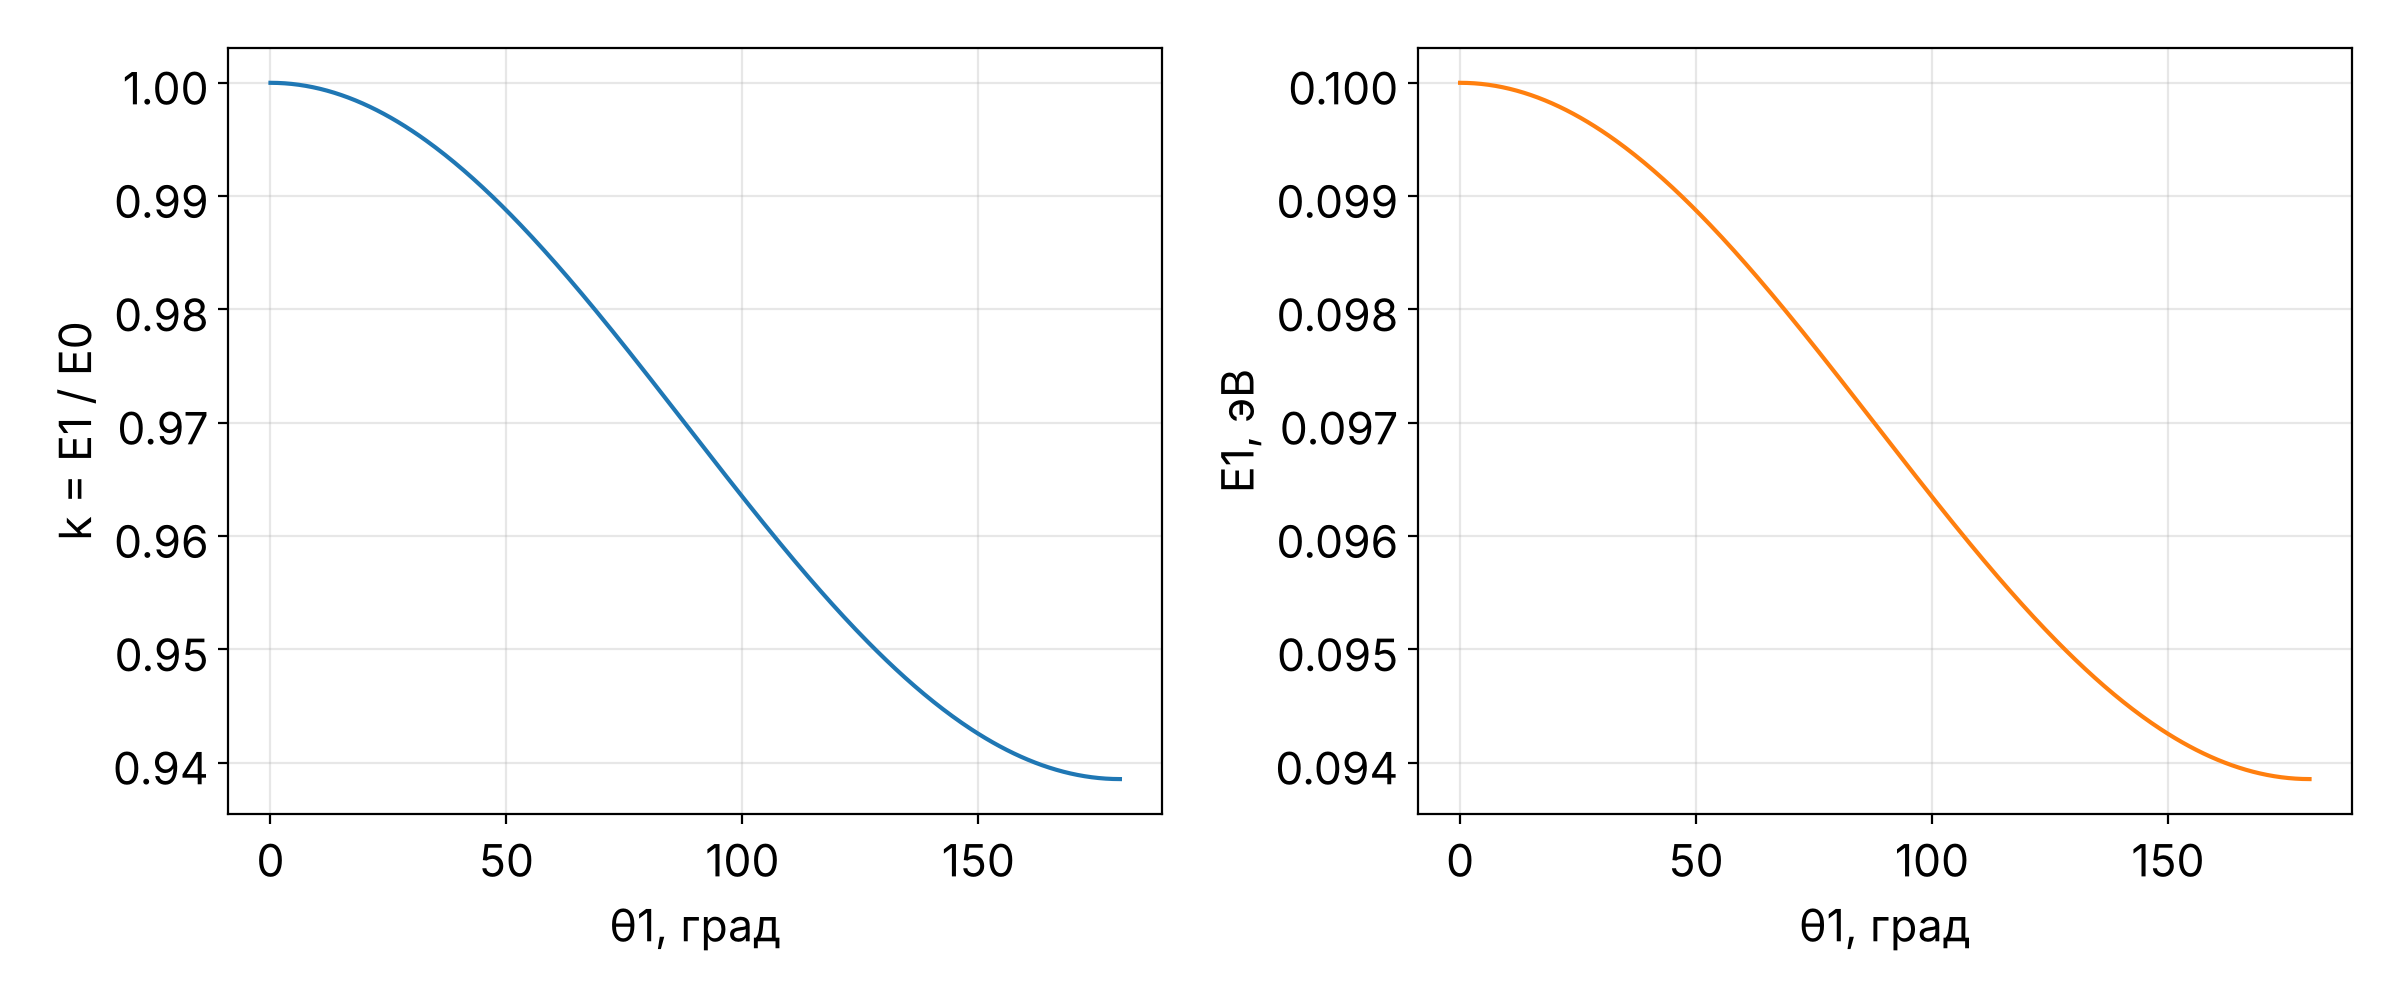
\includegraphics[width=\linewidth]{1b_kinematic_factor.png}
  \caption{Кинематический фактор $k(\theta_1)$ (слева) и энергия протона
    после рассеяния $E_1(\theta_1)$ (справа)}
  \label{fig:kinematic}
\end{figure}

\subsection{Сетка прицельных параметров}

Максимальный прицельный параметр, удовлетворяющий
условию~\eqref{eq:rhomax}, $\rho_{\max} = 0{,}54722$~нм, шаг сетки
$\Delta\rho = 0{,}0027361$~нм. Зависимость расстояния наименьшего сближения
от прицельного параметра приведена на рисунке~\ref{fig:closest}.

\begin{figure}[H]
  \centering
  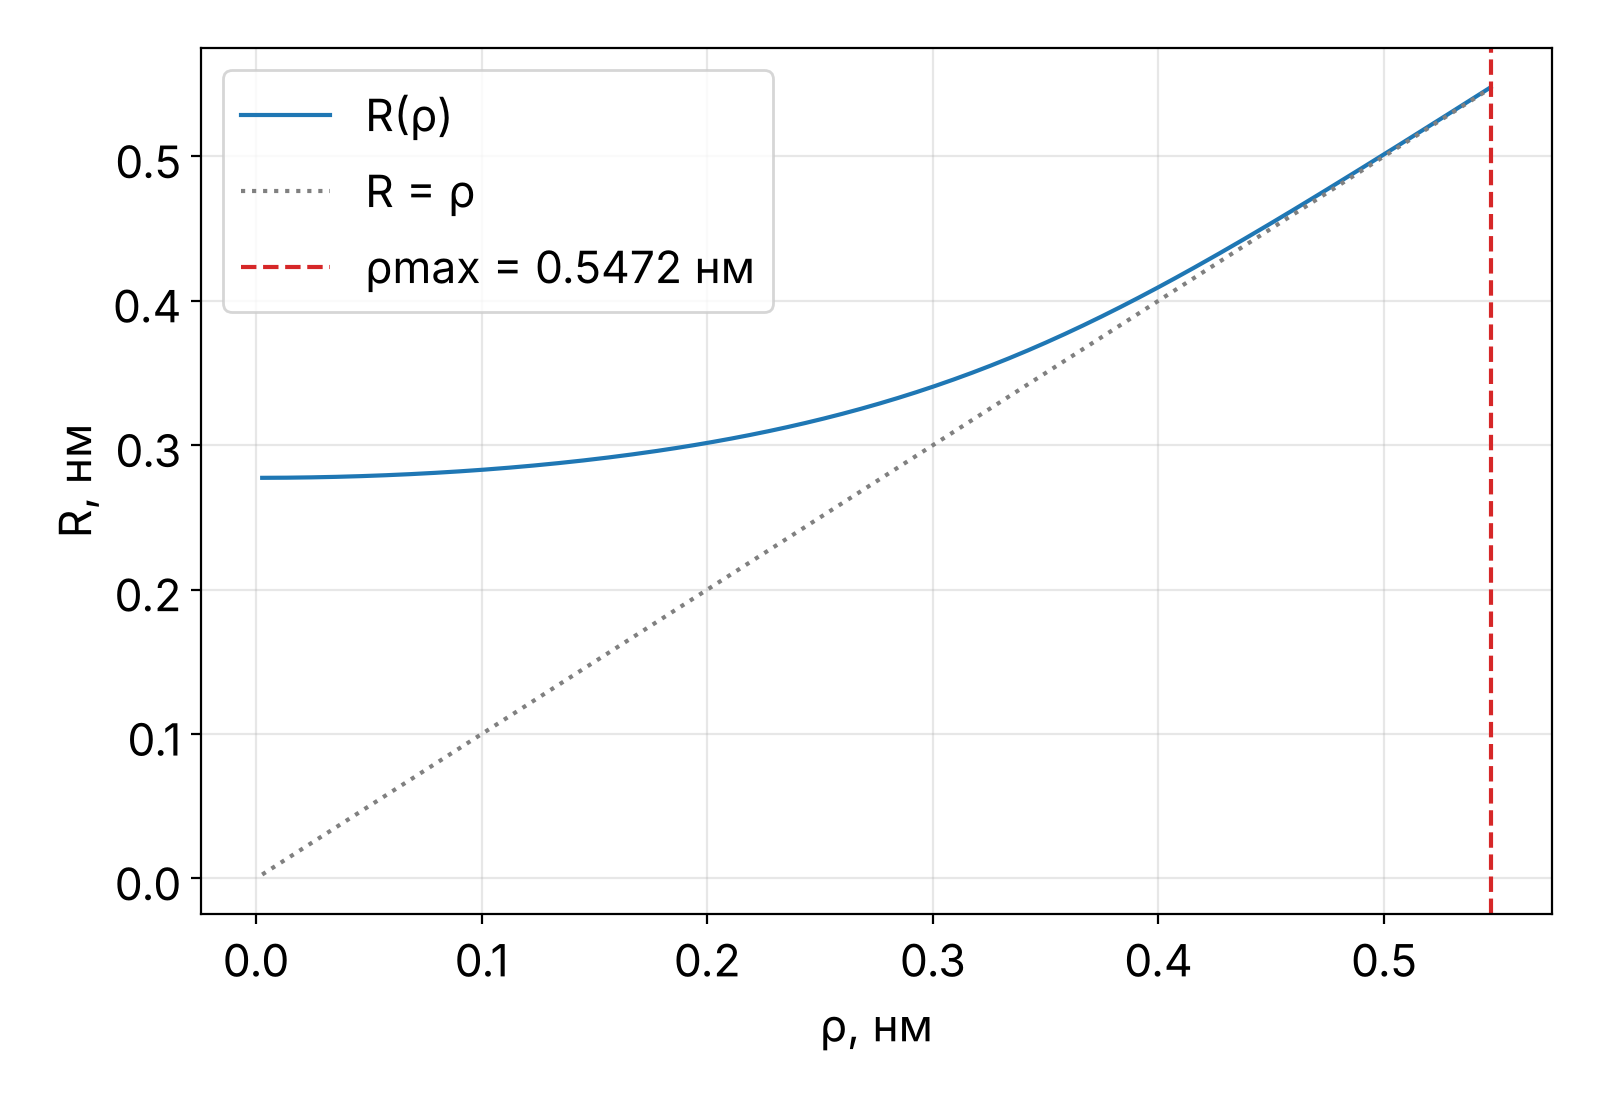
\includegraphics[width=0.85\linewidth]{2_closest_approach.png}
  \caption{Зависимость расстояния наименьшего сближения от прицельного
    параметра}
  \label{fig:closest}
\end{figure}

\subsection{Углы рассеяния}

Зависимости угла рассеяния в ц-системе и углов рассеяния в л-системе
от прицельного параметра приведены на рисунке~\ref{fig:angles}
и в таблице~\ref{tab:results} (приведен каждый двадцатый узел сетки).

\begin{figure}[H]
  \centering
  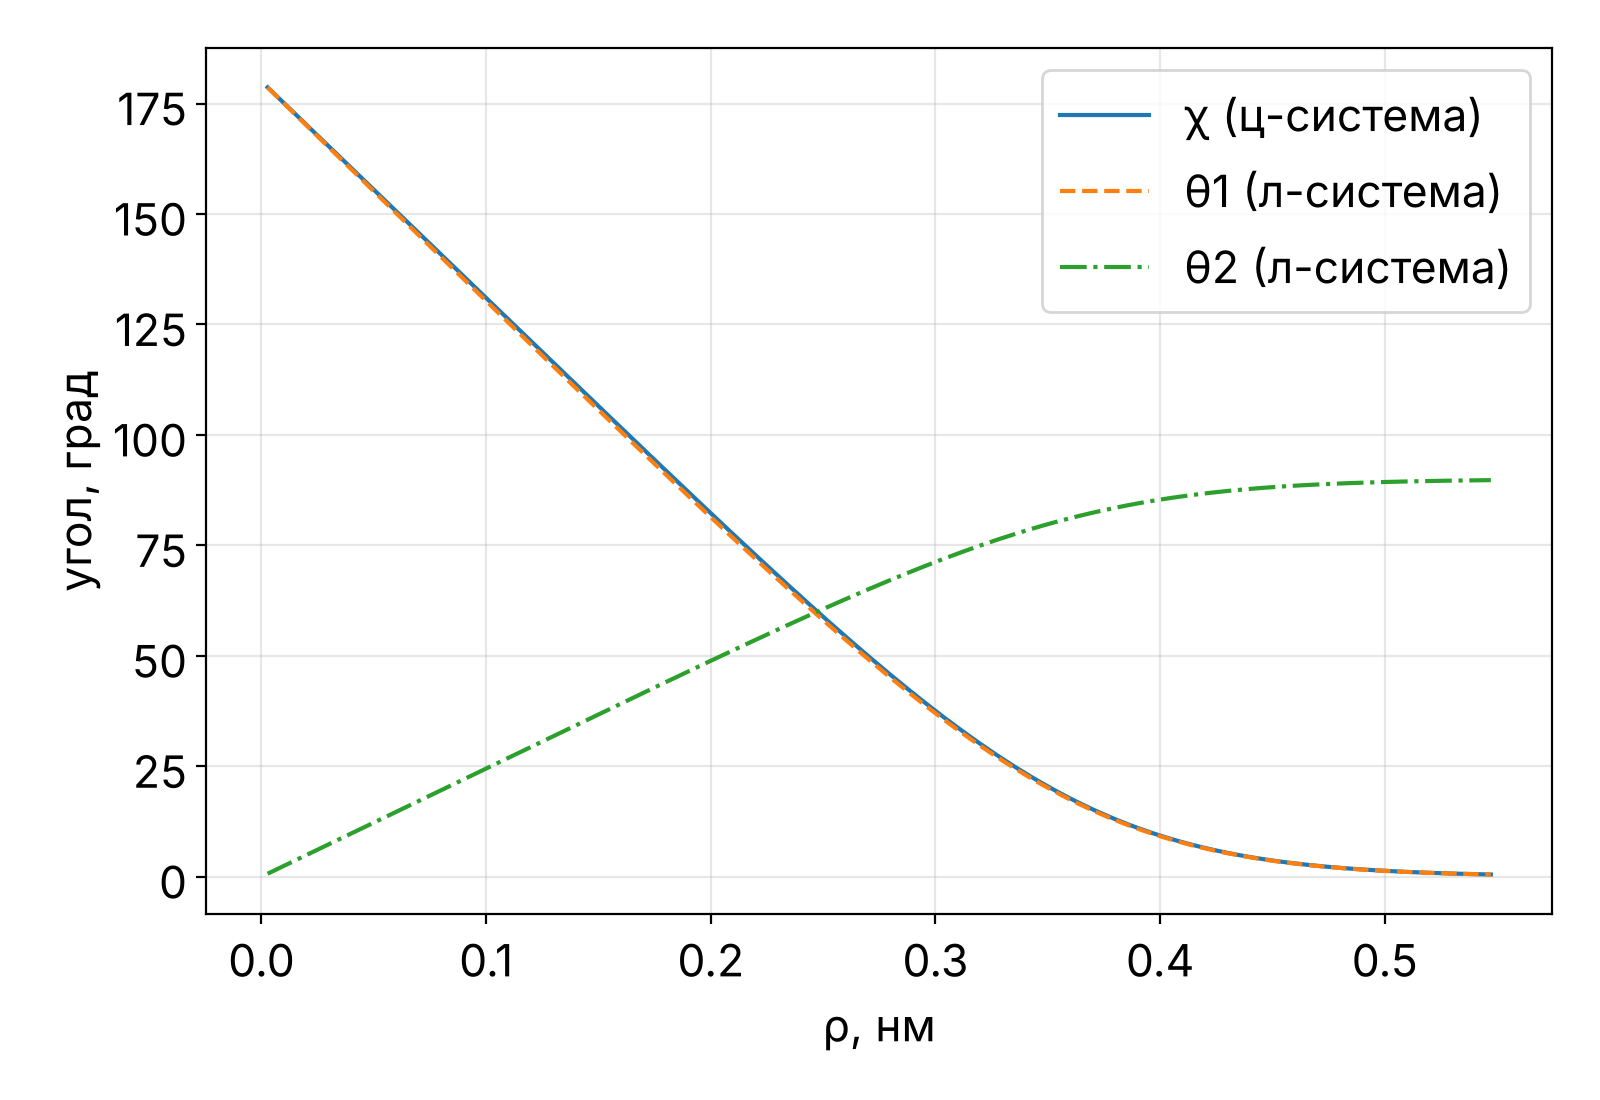
\includegraphics[width=0.85\linewidth]{3_scattering_angles.png}
  \caption{Зависимости углов рассеяния $\chi$, $\theta_1$, $\theta_2$
    от прицельного параметра}
  \label{fig:angles}
\end{figure}

\begin{table}[H]
  \caption{Расстояние наименьшего сближения и углы рассеяния}
  \label{tab:results}
  \setstretch{1}
  \centering
  \begin{tabular}{|c|c|c|c|c|}
    \hline
    $\rho$, нм & $R$, нм & $\chi$, град & $\theta_1$, град & $\theta_2$, град \\ \hline
    \inputrows{generated/results_rows.tex}
  \end{tabular}
\end{table}

\subsection{Дифференциальные сечения рассеяния}

Зависимости прицельного параметра от углов рассеяния в л-системе приведены
на рисунке~\ref{fig:rho}, дифференциальные сечения упругого
рассеяния~--- на рисунке~\ref{fig:sigma}.

\begin{figure}[H]
  \centering
  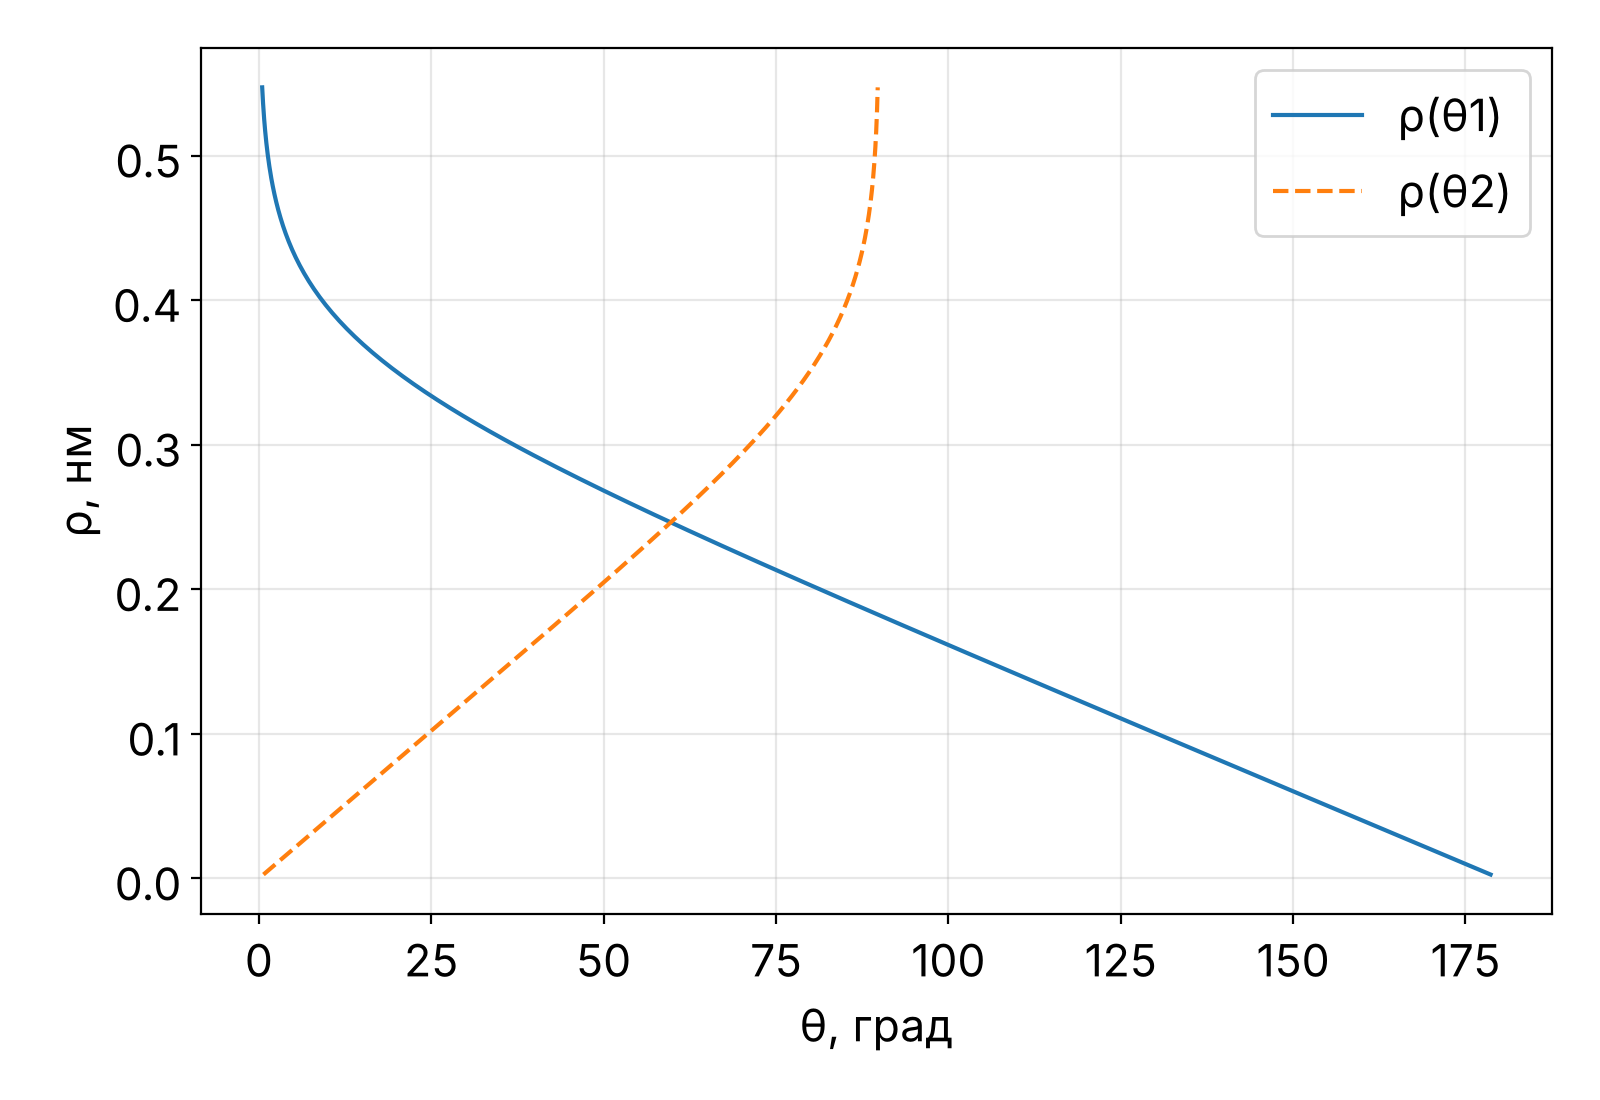
\includegraphics[width=0.85\linewidth]{4a_impact_parameter.png}
  \caption{Зависимости прицельного параметра от углов рассеяния
    $\theta_1$ и $\theta_2$}
  \label{fig:rho}
\end{figure}

\begin{figure}[H]
  \centering
  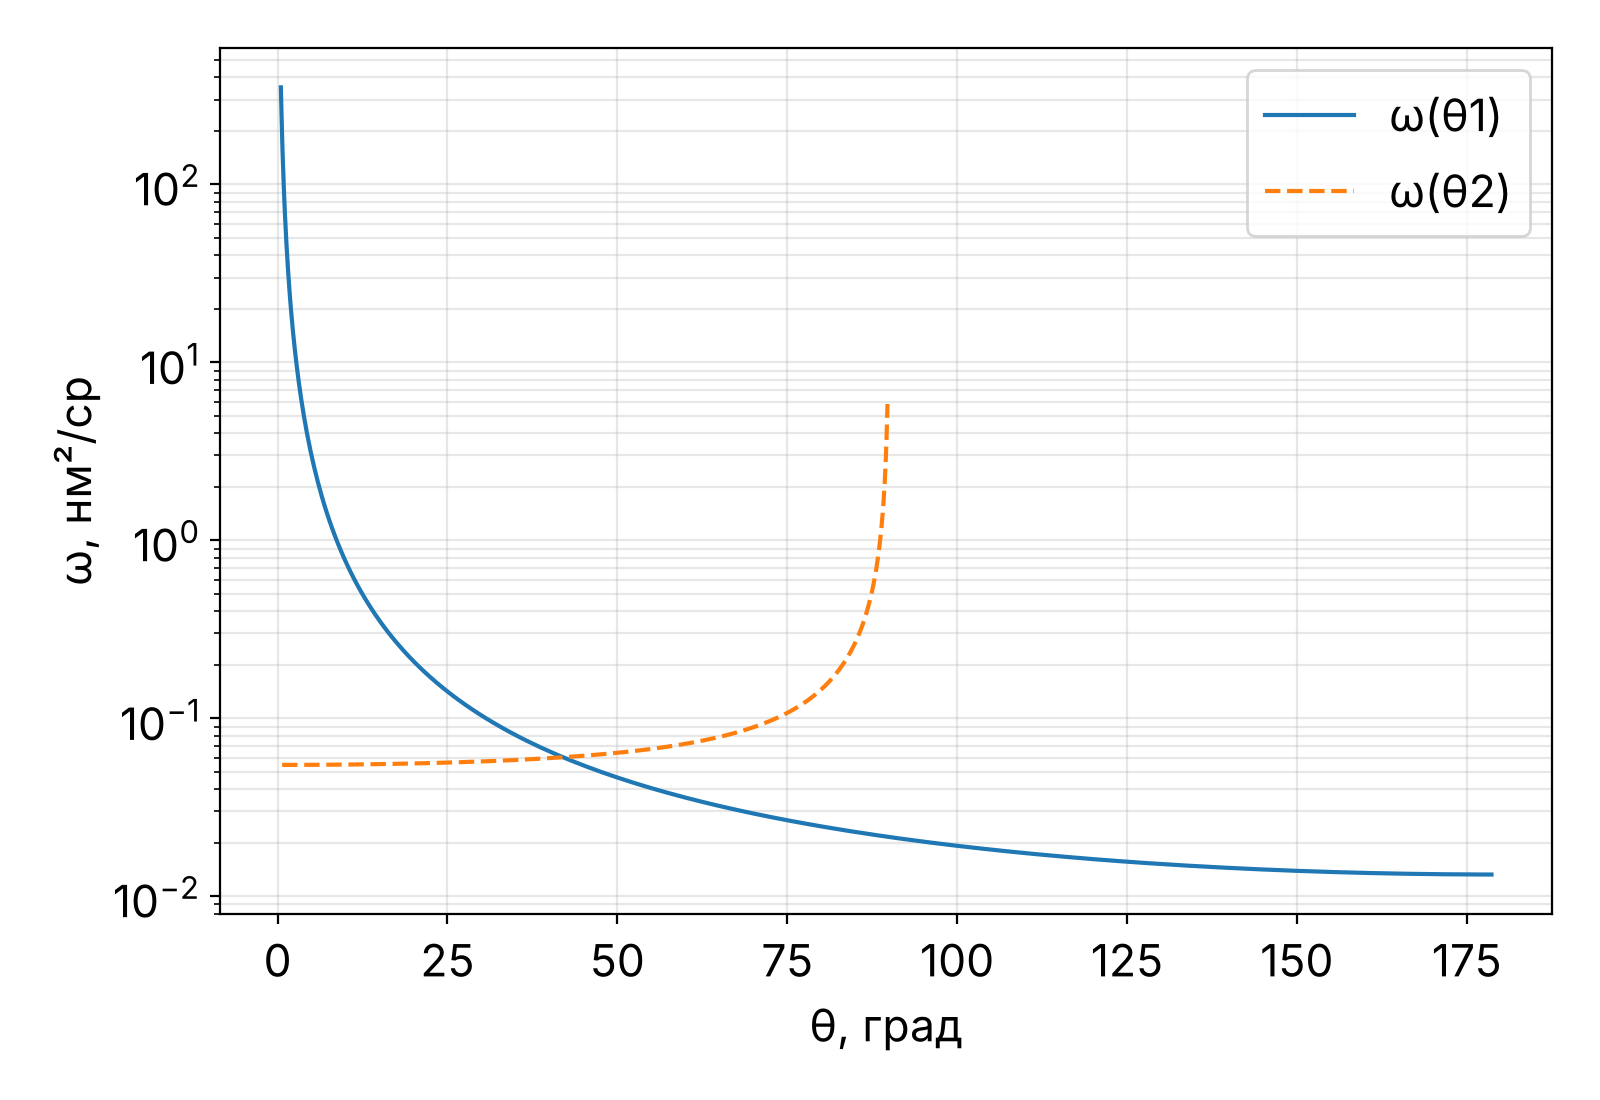
\includegraphics[width=0.85\linewidth]{4b_cross_sections.png}
  \caption{Дифференциальные сечения упругого рассеяния
    $\omega(\theta_1)$ и $\omega(\theta_2)$}
  \label{fig:sigma}
\end{figure}

% ======================== 7 АНАЛИЗ РЕЗУЛЬТАТОВ ===============================
\section{Анализ результатов}

Масса атома меди в 63 раза больше массы протона, поэтому центр масс
системы практически совпадает с атомом мишени: $E_r$ отличается от $E_0$
на 1,6~\%, угол рассеяния в л-системе $\theta_1$ отличается от угла $\chi$
не более чем на $0{,}91^\circ$, а кинематический фактор близок к единице
(протон теряет при упругом столкновении не более 6,1~\% энергии).
Угол вылета атома отдачи $\theta_2 = (\pi - \chi)/2$ не превышает $90^\circ$.

При энергии 0,1~эВ протон отражается на расстоянии около $20\,a_\text{Ф}$
от ядра, где экранированный потенциал убывает практически экспоненциально:
при уменьшении расстояния от 0,4 до 0,28~нм потенциальная энергия возрастает
приблизительно в 17 раз (рисунок~\ref{fig:potential}). Поэтому расстояние
наименьшего сближения слабо зависит от прицельного параметра: при
увеличении $\rho$ от 0 до 0,2~нм оно возрастает лишь на 9~\%
(рисунок~\ref{fig:closest}). Атом мишени ведет себя подобно жесткой сфере
радиусом около 0,28~нм с ``размытой'' поверхностью: угол рассеяния
$\chi(\rho)$ почти линейно убывает от $180^\circ$ до $50^\circ$ при росте
$\rho$ до 0,27~нм (рисунок~\ref{fig:angles}).

При $\rho > 0{,}4$~нм частица пролетает в области, где $U(r) \ll E_r$,
поэтому $R \to \rho$, а угол рассеяния быстро стремится к нулю
(при $\rho = 0{,}44$~нм $\chi = 4{,}6^\circ$, при $\rho = \rho_{\max}$
$\chi = 0{,}49^\circ$). Это и определяет вид дифференциальных сечений
(рисунок~\ref{fig:sigma}):
\begin{itemize}
  \item сечение $\omega(\theta_1)$ резко возрастает при малых углах
        (0,76~нм$^2$/ср при $\theta_1 = 10^\circ$) и слабо зависит от угла при
        рассеянии назад (от 0,022~нм$^2$/ср при $90^\circ$ до 0,013~нм$^2$/ср
        при $170^\circ$), что близко к сечению рассеяния на жесткой сфере
        $R(0)^2/4 = 0{,}019$~нм$^2$/ср;
  \item сечение $\omega(\theta_2)$ почти постоянно при малых углах вылета
        атома отдачи (0,055~нм$^2$/ср при $\theta_2 = 10^\circ$) и резко
        возрастает при $\theta_2 \to 90^\circ$, что соответствует
        скользящим столкновениям с малой передачей энергии.
\end{itemize}

Неограниченный рост сечений при $\theta_1 \to 0$ и $\theta_2 \to 90^\circ$
является особенностью классического описания рассеяния~\cit{ref:manual}
и обусловлен большими прицельными параметрами; в расчете он ограничен
выбором $\rho_{\max}$.

% ================================ ЗАКЛЮЧЕНИЕ =================================
\structuralelement{ЗАКЛЮЧЕНИЕ}

В ходе выполнения практической работы решена задача упругого рассеяния
протона на атоме меди при энергии 0,1~эВ с экранированным кулоновским
потенциалом Kr-C и радиусом экранирования Фирсова.

Разработана объектно"=ориентированная программа на языке Python, в которой
потенциалы, функции и радиусы экранирования, кинематика столкновения,
численные методы и вариант задания представлены отдельными классами.
Программа позволяет выполнить расчет для любого из 24 вариантов задания.

Корректность программы подтверждена сравнением с точным решением задачи
рассеяния в кулоновском поле: погрешность угла рассеяния при 100 узлах
квадратуры Гаусса~--~Мелера не превышает $3{,}2\cdot 10^{-5}$~рад
и убывает пропорционально $1/N^2$.

Получены следующие результаты:
\begin{itemize}
  \item радиус экранирования Фирсова $a_\text{Ф} = 0{,}013608$~нм,
        энергия в ц-системе $E_r = 0{,}098440$~эВ;
  \item расстояние наименьшего сближения при лобовом столкновении
        0,2774~нм, максимальный прицельный параметр
        $\rho_{\max} = 0{,}5472$~нм;
  \item кинематический фактор изменяется от 1 до 0,9386;
  \item рассчитаны зависимости $\chi(\rho)$, $\theta_1(\rho)$,
        $\theta_2(\rho)$ и дифференциальные сечения $\omega(\theta_1)$,
        $\omega(\theta_2)$.
\end{itemize}

При малой энергии столкновения рассеяние протона на атоме меди близко
к рассеянию на жесткой сфере радиусом около 0,28~нм: вероятность рассеяния
на большие углы слабо зависит от угла, а при малых углах сечение резко
возрастает.

% ===================== СПИСОК ИСПОЛЬЗОВАННЫХ ИСТОЧНИКОВ ======================
\structuralelement{СПИСОК ИСПОЛЬЗОВАННЫХ ИСТОЧНИКОВ}

\begin{enumerate}[label=\arabic*., wide=\parindent]
  \item \label{ref:manual}
    Имитационное моделирование плазменных процессов : учебное пособие.~---
    Москва : НИУ «МЭИ», 2025.~--- 110~с.
  \item \label{ref:landau}
    Ландау, Л.\,Д. Теоретическая физика : в 10~т. Т.~1. Механика /
    Л.\,Д.~Ландау, Е.\,М.~Лифшиц.~--- 5-е изд., стер.~--- Москва :
    Физматлит, 2004.~--- 224~с.
  \item \label{ref:eckstein}
    Экштайн, В. Компьютерное моделирование взаимодействия частиц
    с поверхностью твердого тела : пер. с англ. / В.~Экштайн.~---
    Москва : Мир, 1995.~--- 321~с.
  \item \label{ref:krc}
    Wilson, W.\,D. Calculations of nuclear stopping, ranges, and straggling
    in the low-energy region / W.\,D.~Wilson, L.\,G.~Haggmark,
    J.\,P.~Biersack // Physical Review~B.~--- 1977.~--- Vol.~15, no.~5.~---
    P.~2458--2468.
  \item \label{ref:python}
    Python 3 documentation : [сайт].~--- URL: https://docs.python.org/3/
    (дата обращения: 18.10.2026).
  \item \label{ref:numpy}
    Harris, C.\,R. Array programming with NumPy / C.\,R.~Harris,
    K.\,J.~Millman, S.\,J.~van~der~Walt [et~al.] // Nature.~--- 2020.~---
    Vol.~585.~--- P.~357--362.
  \item \label{ref:matplotlib}
    Hunter, J.\,D. Matplotlib: A 2D graphics environment / J.\,D.~Hunter //
    Computing in Science \& Engineering.~--- 2007.~--- Vol.~9, no.~3.~---
    P.~90--95.
  \setcounter{sources}{\value{enumi}}
\end{enumerate}

% ================================ ПРИЛОЖЕНИЕ А ===============================
\appendixsection{А}{Текст программы}

Программа состоит из пакета \texttt{two\_body}, модуля запуска
\texttt{main.py}, модуля тестов \texttt{tests/test\_two\_body.py} и модуля
подготовки рисунков отчета \texttt{report/make\_figures.py}.

\appendixsubsection{Модуль particles.py}
\VerbatimInput{../two_body/particles.py}

\appendixsubsection{Модуль screening.py}
\VerbatimInput{../two_body/screening.py}

\appendixsubsection{Модуль potentials.py}
\VerbatimInput{../two_body/potentials.py}

\appendixsubsection{Модуль kinematics.py}
\VerbatimInput{../two_body/kinematics.py}

\appendixsubsection{Модуль scattering.py}
\VerbatimInput{../two_body/scattering.py}

\appendixsubsection{Модуль cross\_section.py}
\VerbatimInput{../two_body/cross_section.py}

\appendixsubsection{Модуль variants.py}
\VerbatimInput{../two_body/variants.py}

\appendixsubsection{Модуль experiment.py}
\VerbatimInput{../two_body/experiment.py}

\appendixsubsection{Модуль plotting.py}
\VerbatimInput{../two_body/plotting.py}

\appendixsubsection{Модуль \_\_init\_\_.py}
\VerbatimInput{../two_body/__init__.py}

\appendixsubsection{Модуль main.py}
\VerbatimInput{../main.py}

\appendixsubsection{Модуль tests/test\_two\_body.py}
\VerbatimInput{../tests/test_two_body.py}

\appendixsubsection{Модуль report/make\_figures.py}
\VerbatimInput{make_figures.py}

\end{document}
